%+++Art des Dokuments+++++++++++++++++++++++++++++++++++++++++++++++++++++++++++++++++++++++++++++++
\documentclass[a4paper,12pt, DIV12]{scrartcl}

%+++Grundeinstellungen++++++++++++++++++++++++++++++++++++++++++++++++++++++++++++++++++++++++++++++
\usepackage[ngerman]{babel}		%Trennungen, Schriftsatz; Neue deutsche Rechtschreibung
\usepackage[T1]{fontenc}		%Umlaute, Sonderzeichen...				
\usepackage[utf8]{inputenc}		%UTF-8 Support
\usepackage{graphicx}			%Paket um Grafiken einzubinden. Evtl. muss unter Windows  
								% mit \usepackage[dvips]{graphicx} der dvips-Treiber für EPS-Grafiken geladen werden
\usepackage{palatino}			%Schriftart - hier könnte auch times oder helvet stehen
								%wird zwar von l2tabu nicht empfohlen - finde ich persönlich aber
								%die "schönste" Varianten
\usepackage{multicol}			%Paket für mehrspaltige Dokumente
\usepackage{pst-all}			%Paket um pstricks Grafiken darzustellen
\usepackage{float}
\usepackage{longtable}

%+++Glossar+++++++++++++++++++++++++++++++++++++++++++++++++++++++++++++++++++++++++++++++++++++++
\usepackage[nonumberlist]{glossaries}

% alle Begriffe des Glossars
\newglossaryentry{jee}{name=JEE,description={Java Enterprise Edition},first={Java Enterprise Edition (JEE)}}

\makeglossaries

%+++Kopf- und Fusszeilen++++++++++++++++++++++++++++++++++++++++++++++++++++++++++++++++++++++++++
\usepackage{scrpage2}					%An Koma-Script optimierte Kopfzeilenklasse, jedoch auf gut für
										%andere Dokumentklassen zu verwenden Mit diesem Paket sind auch Kopf-
										%und Fusszeilen möglich, die Unterschiede für rechte und linke Seiten
										%machen (bspw für Bücher)

%Hier folgen die Kopfzeilentexte
\ihead{INSERT}
\chead{}
\ohead{}
\ifoot{INSERT}
\cfoot{}
\ofoot{\pagemark}
% nützlich: \pagemark = Seitenzahl

\setheadsepline{1pt}					%Dicke der Trennlinie Kopfzeile - Text
\setfootsepline{0.5pt}					%Dicke der Trennlinie Fusszeile - Text

\pagestyle{scrheadings}					%gemachte Einstellungen anwenden

%+++Linienabstand+++++++++++++++++++++++++++++++++++++++++++++++++++++++++++++++++++++++++++++++++

\usepackage{setspace}
\onehalfspacing							%1.5 Zeilenabstand; 1 = \singlespacing; 2 = \doublespacing


%+++Absatzeinzug++++++++++++++++++++++++++++++++++++++++++++++++++++++++++++++++++++++++++++++++++
\setlength{\parindent}{1em}			% 1em = Größe, die ein großes M der aktuellen Schrift
									% Platz braucht: Somit ist diese Größe Schriftabhängig
									% (was auch Sinn macht)

%Schusterjungen und Hurenkinder vermeiden 
\clubpenalty=5000\relax 
\widowpenalty=5000\relax 
%Maximalwert ist 10000

%+++Hier beginnt das eigenliche Dokument++++++++++++++++++++++++++++++++++++++++++++++++++++++++++ 
\begin{document}
  %---Titelseite------------------------------------------------------------------------------------

\newcommand{\HRule}{\rule{\linewidth}{0.5mm}}

\begin{titlepage}
 
\begin{center}
 
 
% Upper part of the page
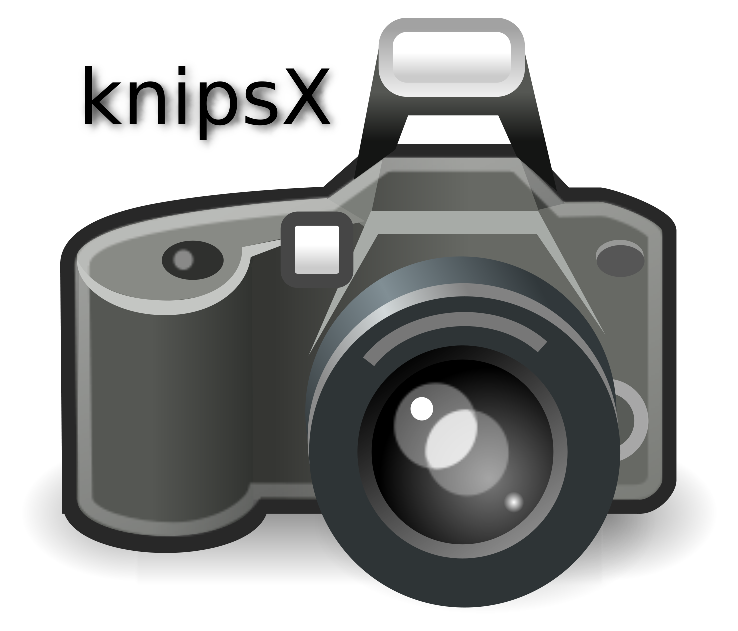
\includegraphics[width=0.33\textwidth]{images/cover.eps}\\[3cm]
 
\textsc{\LARGE Praxis der Softwareentwicklung}\\[1.5cm]
 
\textsc{\Large Gruppe 30 }\\[0.5cm]
 
 
% Title
\HRule \\[0.4cm]
{ \huge \bfseries knipsX}\\[0.4cm]
 
\HRule \\[1.5cm]
 
% Author and supervisor
\begin{minipage}{0.4\textwidth}
\begin{flushleft} \large

Gruppenmitglieder: \\
Borovik, Volodymyr \\
Bouché, Kai \\
Draxler, Benjamin \\
Kaufman, David \\
Zuber, Kevin

\end{flushleft}
\end{minipage}
\begin{minipage}{0.4\textwidth}
\begin{flushright} \large
Gruppenbetreuer: \\
Meder, David
\end{flushright}
\end{minipage} 
\vfill

% Bottom of the page
{\large \today ~- Revision: 1.0}
 
\end{center}
\end{titlepage} \newpage
  \tableofcontents \newpage
  \section{Zielbestimmungen}

\begin{itemize}
  \item Fotografen sollen durch das Produkt in der Lage sein, aus Metadaten ihrer Bilder, welche dem \gls{exif}-Standard entsprechen, Statistiken über ihre Einstellungen beim Fotografieren zu erstellen, diese zu präsentieren sowie sie zu analysieren.
\end{itemize} 

\subsection{Musskriterien}

\label{subsec:musskriterien}

\begin{itemize}
	\item Verwaltung von Projekten
	\item Verwaltung von Bildmengen in Projekten
	\item Verwaltung von Auswertungen
	\item Auslesen, Anzeigen und Auswerten von \gls{exif}-Parametern\\\\
				Auszuwertende \gls{exif}-Parameter sind:
				\label{subsec:auszuwertendedaten}
				\begin{itemize}
					\item Kameramodel
					\item Blitz
					\item Blende 
					\item Verschlusszeit
					\item ISO-Wert
					\item Brennweite
					\item Datum
					\item Wochentag
					\item Uhrzeit
					\item Objektivname
				\end{itemize}
	\item Hinzufügen von Bildern zu Bildmengen per Dateidialog und \gls{dragndrop}
	\item Entfernen von Bildern aus Bildmengen
	\item Bei der Bildauswahl, müssen Vorschaubilder angezeigt werden
	\item Beibehalten von ausgewählten Bildmengen nach Programmbeendigung
	\item Filterung von Bilder anhand von \gls{exif}-Keywords
	\item Vergleich mehrere Bildmengen in einer Auswertung
	\item Erstellen und Anzeigen von verschieden Diagrammtypen aus Bildmengen\\\\
				Notwendige Diagrammtypen:
				\begin{itemize}
					\item Tabelle
					\item 2D Histogramm
					\item 3D Histogramm
					\item Punktewolke
					\item Boxplot \& Unterstützung des Wilcoxon-Mann-Whitney-Tests
				\end{itemize}
	\item Exportieren bzw. Speichern von Diagrammen in Bilder im \gls{jpg}-Format
	\item Das Programm muss in Java 1.6 geschrieben sein
\end{itemize}

\subsection{Wunschkriterien} 

\subsubsection{Hohe Priorität}

	\begin{itemize}
		\item Internationalisierungsmechanismen vorbereiten
		\item Anzeige der Bildliste einschränkbar durch Auswahl in der Inhaltsliste
		\item weiter Ausgabeformate unterstützen 
		\item Einstellung der Größe der Thumbnails in der Projektansicht mittels eines Schiebereglers
	\end{itemize}

\subsubsection{Mittlere Priorität}

	\begin{itemize}
		\item Optimierung von Algorithmen
		\item Anzeige von Thumbnails sowie Dateinamen in Diagrammen über eine Mengenauswahl
		\item Vernünftige eventuell anpassbare Diagrammskalierungen
		\item Konfigurierbarkeit des Layouts	
	\end{itemize}

\subsubsection{Niedrige Priorität}

	\begin{itemize}
		\item Unterstützen weiterer \gls{exif}-Parameter sowie Kameraspezifischer Parameter
		\item Normierung von Werten, z.B. Brennweitenkorrektur
		\item Unterstützung weiterer Bildformate mit Metadaten 	
		\item Weitere Diagrammtypen
	\end{itemize}

\subsection{Abgrenzungskriterien} 
\begin{itemize}
	\item \gls{tempX} soll keine \gls{exif} Daten bearbeiten können.
	\item \gls{tempX} soll keine Bilder bearbeiten bzw. löschen können.
	\item \gls{tempX} soll keine Bilder ausdrucken können.
	\item \gls{tempX} soll keine Diashow anzeigen können.
	\item \gls{tempX} muss keinen hohen Sicherheitsansprüchen genügen.
\end{itemize} \newpage
  \section{Produkteinsatz}
  \begin{itemize}
  \item Das Produkt dient zur Untersuchung des Nutzungsverhaltens von Hobby- als auch Profifotografen mittels Statistiken. \gls{tempX} ist Open Source (siehe Anhang \ref{subsec:gpl}).
  \end{itemize}
\subsection{Anwendungsbereiche}
  \begin{itemize}
  \item Fotografie
  \end{itemize}

\subsection{Zielgruppe}
	\begin{itemize}
		\item Hobby- sowie Freizeitfotografen
		\item Profifotografen		
	\end{itemize}

\subsection{Betriebsbedingungen}
  \begin{itemize}
  		\item Zuhause oder am Arbeitsplatz. Das Produkt ist für herkömmliche moderne Desktop-PCs vorgesehen.
  \end{itemize}
 \newpage
  \section{Produktumgebung}

Das Programm l�uft auf einem der Poolrechner im Raum 356 des Informatik Geb�udes 50.34 des Karlsruher Institut of Technologies.

\begin{itemize}
\item Software
	\begin{itemize}
	\item Betriebssystem: 
		\begin{itemize}
			\item Windows 2000/XP/Vista/7
			\item Linux
			\item (optional) Mac OS X 10.5
		\end{itemize}
	
	\item Laufzeitumgebung:
		\begin{itemize}
			\item Java 1.6
		\end{itemize}		
	\end{itemize}
	
\item Hardware 
	\begin{itemize}
	\item Mindestanforderung an den Arbeitsplatzrechner: 
		\begin{itemize}
			\item Dual Core 2 Ghz
			\item 2 GB RAM
			\item Bildschirm mit einer Aufl�sung von 800 x 600 Pixel
			\item Hardbwarebeschleunigte 3D Unterst�tzung
		\end{itemize}
	
	\item Kamera:
		\begin{itemize}
			\item Alle Kameramodelle die mindestens den JEITA Exif Version 2.1 Standard vom 1. Juni 1998 einhalten
		\end{itemize}		
	\end{itemize}	
\end{itemize} \newpage
  \section{Funktionale Anforderungen}

\subsection{Programmausführung}

\label{subsec:programmausfuehrung}

	\begin{description}
		
		\item[/F010/] \textit{Programm beenden:}\par In der Projektansicht und der Projektübersicht ist die Möglichkeit gegeben durch betätigen der "`Fenster schließen"' Schaltfläche (differiert je nach Betriebssystem), das Programm zu beenden.
		
		\item[/F020/] \textit{Speicherverhalten:}\par Nach jedem Dialog ist die Möglichkeit gegeben, die aktuelle Änderung für die aktuelle Programmausführung zu übernehmen. Sollen Änderungen dauerhaft gesichert werden, muss die Schaltfläche "`Speichern"' in dem Bereich "`Projekt"' der Projektansicht betätigt werden. Dadurch, wird die Projektkonfigurationsdatei neu generiert und in dem Projektverzeichnis gespeichert.
		
		\item[/F030/] \textit{Automatische Anpassung der Größe der Bedienoberfläche:}\par Das Programm positioniert automatisch seine Bedienelemente, in Abhängigkeit zur Auflösung des Programmfensters.
		
		\item[/F040/] \textit{Automatisches durchsuchen des Projektverzeichnisses:}\par Bei Programmstart, wird in dem Projektverzeichnis des Programms nach Projektkonfigurationsdateien gesucht. Auf der Basis dieser Datensätze wird eine Projektliste generiert, die in einem Projektübersicht, nach absteigendem Bearbeitungsdatum (aktuelles zuerst), sortiert angezeigt werden. Zudem wird das Datum anders formatiert dargestellt als der Projektname.
		
	\end{description}

\subsection{Projektmanagement}

\label{subsec:projektmanagement}
	
	\gls{tempX} verfügt über eine eingebaute Projektverwaltung, mit der der Benutzer beliebige Kombinationen von Bildmengen und Auswertungen verwalten kann. Es kann allerdings immer nur ein Projekt im aktiven Zustand sein, ein Wechsel in ein anderes Projekte während der Programmausführung ist möglich.\par Ein Projekt wird in einer Projektkonfigurationsdatei gespeichert, die sich in dem Projektverzeichnis von \gls{tempX} befindet. Dieses Projektverzeichnis ist vom Elternverzeichnis ausgehend mit "`projekte"' gekennzeichnet.
	
	\begin{description}		
		
		\item[/F110/] \textit{Neues Projekt anlegen:}\par In der Projektübersicht ist die Möglichkeit gegeben, durch betätigen der Schaltfläche "`Projekt erstellen"', ein neues Projekt zu erstellen und ihm einen Namen zu geben.\par Dabei wird überprüft, ob dieser Projektname schon von einem anderen Projekt verwendet wird. Ist dies der Fall, kann der Benutzer einen neuen Namen eingeben. Dabei ist auch zu beachten, dass der Projektname zwischen einem und 255 Zeichen lang sein muss.\par Bei der Projektanlegung wird auch ein Erstellungsdatum erstellt (siehe Kapitel \ref{subsec:programmdaten} \textbf{/D20/}). Danach wird die Projektansicht gestartet, mit dem gerade erstellten Projekt (siehe Kapitel \ref{subsec:benutzerschnittstelle}). Zu beachten ist, dass ein Projekt erst nach der in Kapitel \ref{subsec:programmausfuehrung} beschriebenen Funktion \textbf{/F020/} dauerhaft verfügbar ist. 
		
		\item[/F120/] \textit{Projekt aktivieren:}\par Um eine Projekt zu aktivieren, muss man es in der Liste der Projekte, in dem Dialog aus \textbf{/F040/}, auswählen.
		
		\item[/F130/] \textit{Vorhandens Projekt öffnen:}\par In der Projektübersicht ist die Möglichkeit gegeben, durch einen Doppelklick, mit der linken Maustaste, auf den Projektnamen eines bereits vorhanden Projektes oder durch aktivieren eines Projektes und betätigen der Schaltfläche "`Projekt öffnen"' (siehe Kapitel \ref{subsec:benutzerschnittstelle}, das Hauptprogramm zu starten.\par In der damit verbundenen Projektkonfigurationsdatei gespeicherte Bildmengen und Auswertungen werden nun verfügbar gemacht. Damit gemeint ist: 
			
			\begin{itemize}
				
				\item Das Einlesen von \gls{exif}-Parametern aller Bilder, die in den Bildmengen des Projekts definiert sind. Das Einlesen geschieht im Hintergrund, d.h. der Benutzer kann mit dem Programm interagieren, vollständige Funktionalität ist aber erst nach dem vollständigen Einlesen der \gls{exif} Daten gegeben.
				
				\item Anzeige der Bildmengen (siehe Kapitel \ref{subsec:bildmengenmgmt} \textbf{/F250/}).
				
				\item Anzeige der Auswertungen (siehe Kapitel \ref{subsec:auswertungsmgmt}).
				
				\item Anzeige aller Bilder der Bildmengen in dem Bereich "`Bildansicht"' und aktivieren des ersten Bildes. Dadurch wird der Bereich "`\gls{exif}-Daten"' der Projektansicht, mit den \gls{exif}-Parametern dieses Bildes aktualisiert.
			
			\end{itemize}		
		
		\item[/F140/] \textit{Projekt kopieren:}\par In der Projektübersicht ist die Möglichkeit gegeben, ein aktiviertes Projekt mit allen in ihm definierten Daten, Bildmengen und Auswertungen zu kopieren und es unter neuem Namen und neuem Erstellungsdatum temporär zu definieren. Danach wird die Projektansicht gestartet, mit dem gerade kopierten Projekt (siehe Kapitel \ref{subsec:benutzerschnittstelle}). Zu beachten ist, dass ein Projekt erst nach der in Kapitel \ref{subsec:programmausfuehrung} beschriebenen Funktion \textbf{/F020/} dauerhaft verfügbar ist.
		
		\item[/F150/] \textit{Projekt entfernen:}\par In der Projektübersicht ist die Möglichkeit gegeben, bei einem aktivierten Projekt mit betätigen der Schaltfläche "`Projekt entfernen"' folgende Aktionen auszulösen:
			
			\begin{enumerate}
				
				\item Es wird eine Sicherheitsabfrage (ein Dialog mit Ja/Nein Auswahlmöglichkeit) angezeigt, die dem Benutzer die Möglichkeit gibt, das Entfernen abzubrechen.
				
				\item Das Projekt wird aus der Liste der Projekte, in der Projektübersicht, entfernt.
				
				\item Die Projektkonfigurationsdatei, wird in dem Projektverzeichnis gelöscht.
				
				\item Dem Benutzer wird eine Rückmeldung gegeben, ob das Entfernen erfolgreich war oder ob es einen Fehler gab.
			
			\end{enumerate}
	
		\item[/F160/] \textit{Projektbeschreibung hinzufügen:}\par in dem Feld "`Projektbeschreibung"' lässt sich das Projekt genauer spezifizieren. Erst nach Ausführung von \textbf{/F020/} ist diese dauerhaft verfügbar.
	
		\item[/F170/] \textit{Projekt wechseln:}\par durch betätigen der Schaltfläche "`Wechseln"' in dem Bereich "`Projekt"' der Projektansicht, werden folgende Aktionen ausgelöst:
		\begin{enumerate}
				
				\item Es wird eine Sicherheitsabfrage (ein Dialog mit Ja/Nein Auswahlmöglichkeit) angezeigt, die dem Benutzer die Möglichkeit gibt, das Projekt zu speichern.
				
				\item Das gerade aktive Projekt wird geschlossen.
				
				\item Die Projektansicht wird beendet.
				
				\item Die Projektübersicht wird gestartet.
			
			\end{enumerate}
	
	\end{description}

\subsection{Bildmengenmanagement}

\label{subsec:bildmengenmgmt}
	
	In einem Projekt, können Bildmengen verwaltet werden (siehe Kapitel \ref{sec:nichtfunktionale_anforderungen} \textbf{/NF020/}). Eine Bildmenge ist folgendermaßen definiert:
	
	\begin{itemize}
		
		\item Eine Bildmenge kann beliebig (im Rahmen der \textbf{/NF020/)} viele Verweise auf Bilder (im \gls{jpg}-Format) des verwendeten Dateisystems enthalten.
		
		\item Eine Bildmenge kann beliebig (im Rahmen der \textbf{/NF020/)} viele Verweise auf Verzeichnisse des verwendeten Dateisystems enthalten.
		
		\item Eine Bildmenge kann beliebig (im Rahmen der \textbf{/NF020/)} viele Verweise auf Bildmengen haben, die in dem Projekt definiert sind. Dabei ist zu beachten:
		
			\begin{itemize}
			
				\item Bei den Verweisen, darf es zu keinen Endlosverweisen führen (Bildmenge A ist in Bildmenge B und Bildmenge B ist in Bildmenge A).
				
				\item Wird eine Bildmenge entfernt, so wird ein Verweis auf diese Bildmenge ebenfalls entfernt.
			
			\end{itemize}
		
		\item Eine Bildmenge hat einen frei definierbaren und vom Projektkontext abhängigen eindeutigen Namen, der zwischen einem und 255 Zeichen lang sein muss.
		
		\item Eine Bildmenge wird über eine interne ID eindeutig identifiziert.
	
	\end{itemize}
	
	Es ist außerdem zu beachten, dass bei einem Dateisystem- oder einem Datenspeicherstrukturwechsel die Verweise keine Gültigkeit mehr haben können und ein Neuanlegen dieser Verweise unumgänglich ist.\par Wird ein Projekt geöffnet, werden alle in der Projektkonfigurationsdatei definierten Bildmengen \gls{lexgraph} sortiert angezeigt. Die erste Bildmenge der Liste (falls vorhanden), wird dabei automatisch auf aktiv gesetzt.
	
	\begin{description}
		
		\item[/F210/] \textit{Anlegen einer neuen Bildmenge:}\par Durch betätigen der Schaltfläche "`Erstellen"' im Bereich "`Bildmengen"' der Projektansicht, wird ein Dialog geöffnet, der dem Benutzer die Möglichkeit gibt, der Bildmenge einen Namen zu geben.
		
		\item[/F220/] \textit{Aktivieren einer Bildmenge:}\par Um eine Bildmenge zu aktivieren, muss man sie in der Liste der Bildmengen, im Bereich "`Bildmengen"' der Projektansicht, auswählen. Dadurch wird der Bereich "`Inhalt"' der Projektansicht aktualisiert (siehe Kapitel \textbf{/F250/}).
		
		\item[/F230/] \textit{Hinzufügen von Bildern und Verzeichnissen zu einer vorhandenen Bildmenge:}\par Um diese Aktionen auszuführen, muss eine Bildmenge aktiv sein. Das Hinzufügen kann über zwei Arten geschehen:
		
			\begin{itemize}
				
				\item Durch \gls{dragndrop} von Verzeichnissen und Bildern aus der grafischen Benutzerschnittstelle des Betriebssystems in den Bereich "`Inhalt"', einer aktiven Bildmenge. 
				
				\item Durch betätigen der Schaltfläche "`Hinzufügen"' in dem Bereich "`Inhalt"' der Projektansicht einer aktiven Bildmenge, wird ein Dialog (der je nach verwendetem Betriebssystem eine unterschiedliche Handhabung hat) geöffnet, der dem Benutzer folgende Möglichkeiten gibt:
				
					\begin{itemize}
			
						\item Auswahl beliebig (im Rahmen der \textbf{/NF020/)} vieler Verzeichnisse, die einzeln als Pfade zum jeweiligen Verzeichnis in die Bildmenge übernommen werden. Ausgehend von diesen Verzeichnissen, wird rekursiv der Verzeichnisbaum nach Bilder im \gls{jpg}-Format durchsucht.
						
						\item Auswahl beliebig (im Rahmen der \textbf{/NF020/)} vieler Bilder im \gls{jpg}-Format, deren Pfade einzeln in die Bildmenge übernommen werden.
					
					\end{itemize}
				
			\end{itemize}
		
		\item[/F240/] \textit{Hinzufügen von Bildmengen zu einer vorhandenen Bildmenge:}\par Das Hinzufügen kann nur per \gls{dragndrop} einer vorhanden Bildmenge aus dem Bereich "`Bildmengen"' der Projektansicht in den Bereich "`Inhalt"' der Projektansicht einer aktiven Bildmenge erfolgen. Dabei wird die Definition von Bildmengen eingehalten (siehe Kapitel \ref{subsec:bildmengenmgmt}).
		
		\item[/F250/] \textit{Entfernen von Bildmengen:}\par Um diese Aktionen auszuführen, muss eine Bildmenge aktiv sein. Durch betätigen der Schaltfläsche "`Entfernen"', werden folgende Aktionen ausgelöst:
			
			\begin{enumerate}
			
				\item Es wird eine Sicherheitsabfrage (ein Dialog mit Ja/Nein Auswahlmöglichkeit) angezeigt, die dem Benutzer die Möglichkeit gibt, das Entfernen abzubrechen.
				
				\item Die Bildmenge wird aus der Liste der Bildmengen, in dem Bereich "`Bildmengen"' der Projektansicht, entfernt.
				
				\item Es werden alle restlichen Bildmengen nach Verweisen auf diese Bildmenge durchsucht. Falls Verweise vorhanden sind, werden diese Verweise entfernt.
				
				\item Dem Benutzer wird eine Rückmeldung gegeben, ob das Entfernen erfolgreich war oder ob es einen Fehler gab.
				
				\item Nach dem Entfernen, ist die erste Bildmenge (falls vorhanden) in der Liste aktiv.
			
			\end{enumerate}

		\item[/F260/] \textit{Aufbau der Inhaltsliste:}\par Ist eine Bildmenge aktiv, wird in dem Bereich "`Inhalt"' der Proektansicht die Liste mit dem Inhalt der Bildmenge aktualisiert. Die Liste wird dabei blockweise nach folgendem Schema aufgebaut:
		
			\begin{enumerate}
			
				\item Mit der Bildmenge verknüpfte Bildmengen, \gls{lexgraph} sortiert.
			
				\item Mit der Bildmenge verknüpfte Verweise auf Verzeichnise, \gls{lexgraph} sortiert.
				
				\item Mit der Bildmenge verknüpfte Verweise auf Bilder, \gls{lexgraph} sortiert.
				
			\end{enumerate}
			
			Jeder Block ist dabei mit einer unterschiedlichen Textfarbe formatiert.
		
	\end{description}

\subsection{Diagrammmanagement}

\label{subsec:diagrammmgmt}

	\gls{tempX} beherrscht verschiedene Diagrammtypen, welche im folgenden genannt sind:
	
	\begin{description}

		\item[/F310/] \textit{Tabelle:}\par 
		
			\begin{figure}[H]
				\centering
				\fbox{
					\begin{minipage}{13 cm}
						\centering
						\resizebox{13 cm}{!} {
\begin{tabular}{|c|c|c|c|c|c|c|}
\hline  Name & Manufacturer & Date and Time & FNumber & Exposure Time & Flash \\ 
\hline  DSC00601.JPG & Sony Ericsson   & 2009:11:07 00:27:48  & f/2,8 & 1/1000 & False\\ 
\hline  DSC00602.JPG & Sony Ericsson & 2009:11:06 10:27:26 & f/2,8  & 1/1600 & False \\ 
\hline  DSC00606.JPG & Sony Ericsson & 2009:11:06 12:35:59 & f/2,8  & 1/800 & False \\ 
\hline  SDC16734.JPG & Samsung Techwin & 2009:11:05 00:59:01   & f/7,0 & 1/250 & False\\ 
\hline  SDC16742.JPG & Samsung Techwin & 2009:11:06 05:52:36   & f/7,1 & 1/250 & False\\ 
\hline 
\end{tabular} 

}
						\caption{Ansicht einer tabellarischen Auswertung}
						\label{diag:tabelle}
					\end{minipage}  
				}    		
			\end{figure}			
			Die Tabelle stellt alle auszuwertenden \gls{exif}-Daten mit Dateinamen tabellarisch dar (siehe Kapitel \ref{subsec:auszuwertendedaten}). Dabei wird \gls{lexgraph} nach dem Dateinamen sortiert. Die Tabelle kann als \gls{jpg} exportiert werden.

		\item[/F320/] \textit{2D Histogramm:}\par 
		
			\begin{figure}[H]
				\centering
				\fbox{
					\begin{minipage}{13 cm}
						\centering						
						% Generated with LaTeXDraw 2.0.2
% Tue Nov 17 17:42:28 CET 2009
% \usepackage[usenames,dvipsnames]{pstricks}
% \usepackage{epsfig}
% \usepackage{pst-grad} % For gradients
% \usepackage{pst-plot} % For axes
\scalebox{1} % Change this value to rescale the drawing.
{
\begin{pspicture}(0,-3.6579165)(12.652083,3.6979167)
\definecolor{color2405b}{rgb}{0.3764705882352941,0.6666666666666666,0.9921568627450981}
\rput(0.74583334,-2.9120834){\psaxes[linewidth=0.04,ticksize=0.10583333cm,dx=1.15cm,dy=1.0cm,Dx=100]{->}(0,0)(0,0)(11,6)}
\psframe[linewidth=0.04,dimen=outer,fillstyle=solid,fillcolor=color2405b](1.9058334,1.1079167)(0.72583336,-2.9320834)
\psframe[linewidth=0.04,dimen=outer,fillstyle=solid,fillcolor=color2405b](3.0658333,0.10791667)(1.8658333,-2.9320834)
\psframe[linewidth=0.04,dimen=outer,fillstyle=solid,fillcolor=color2405b](4.2658334,-0.89208335)(3.0258334,-2.9320834)
\psframe[linewidth=0.04,dimen=outer,fillstyle=solid,fillcolor=color2405b](5.3658333,0.10791667)(4.175833,-2.9320834)
\psframe[linewidth=0.04,dimen=outer,fillstyle=solid,fillcolor=color2405b](6.565833,-1.8920833)(5.3258333,-2.9320834)
\psframe[linewidth=0.04,dimen=outer,fillstyle=solid,fillcolor=color2405b](7.6658335,0.10791667)(6.465833,-2.9320834)
\psframe[linewidth=0.04,dimen=outer,fillstyle=solid,fillcolor=color2405b](8.825833,2.1079166)(7.6258335,-2.9320834)
\psframe[linewidth=0.04,dimen=outer,fillstyle=solid,fillcolor=color2405b](9.965834,0.10791667)(8.785833,-2.9320834)
\psframe[linewidth=0.04,dimen=outer,fillstyle=solid,fillcolor=color2405b](11.105833,-0.89208335)(9.925834,-2.9320834)
\usefont{T1}{ptm}{m}{n}
\rput(12.324427,-2.8220832){ISO}
\usefont{T1}{ptm}{m}{n}
\rput(0.73067707,3.5179167){Anzahl}
\psline[linewidth=0.04cm,linestyle=dashed,dash=0.16cm 0.16cm](0.8858333,2.0879166)(11.885834,2.0879166)
\psline[linewidth=0.04cm,linestyle=dashed,dash=0.16cm 0.16cm](0.8858333,1.0879166)(11.885834,1.0879166)
\psline[linewidth=0.04cm,linestyle=dashed,dash=0.16cm 0.16cm](0.8858333,0.087916665)(11.885834,0.087916665)
\psline[linewidth=0.04cm,linestyle=dashed,dash=0.16cm 0.16cm](0.8858333,-0.9120833)(11.885834,-0.9120833)
\psline[linewidth=0.04cm,linestyle=dashed,dash=0.16cm 0.16cm](0.8858333,-1.9120834)(11.885834,-1.9120834)
\end{pspicture} 
}

						\caption{Ansicht eines 2D Histogramms}
						\label{diag:2dhistogramm}
					\end{minipage}  
					}    		
			\end{figure}
			Das 2D Histogramm gibt eine grafische Darstellung der Häufigskeitsverteilung von Messwerten an. Dabei wird ein \gls{exif}-Parameter der X-Achse zugewiesen, die in äquidistante Abschnitte zerlegt wird. Die Y-Achse gibt die Häufigkeit des zu betrachtenden Abschnittes an. Falls n Bildmengen mit der aktuellen Auswertung verbunden sind, so wird jeder Abschnitt nochmals in n gleich große Unterabschnitte zerlegt ($ n \in \mathbb{N} $ und $ n>1 $). Das 2D Histogram kann als \gls{jpg} exportiert werden.
			

		\item[/F330/] \textit{3D Histogramm:}\par
			
			\begin{figure}[H]
				\centering
				\fbox{
					\begin{minipage}{13 cm}
						\centering
						\resizebox{113 mm}{!} {
							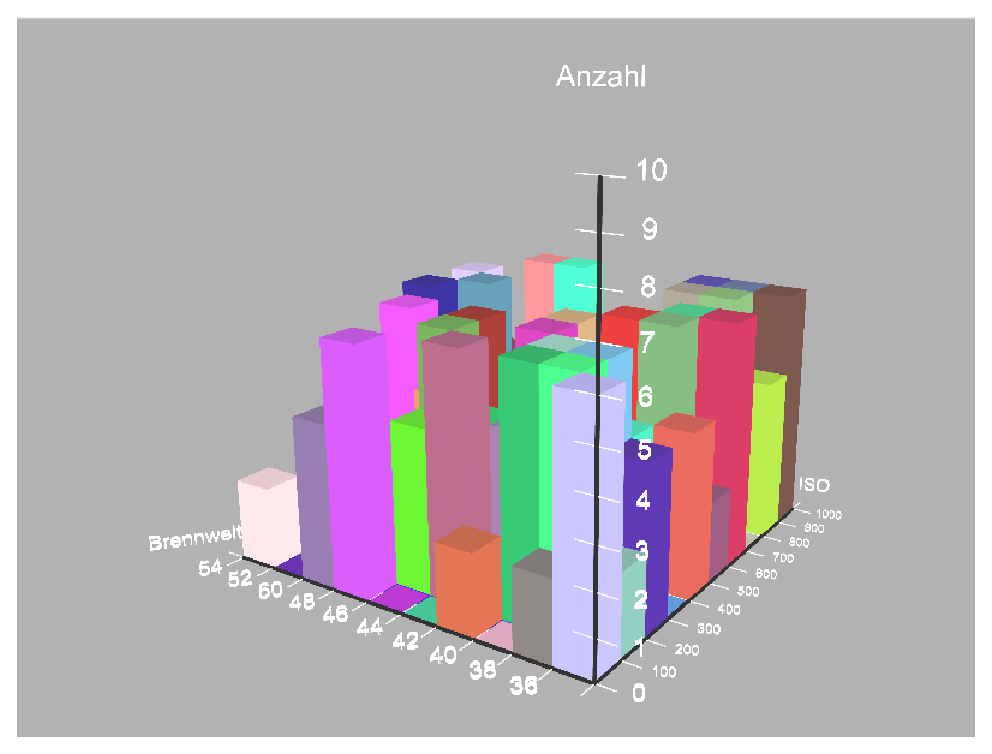
\includegraphics{images/3DHistogramm.eps}
						} 
						\caption{Ansicht eines 3D Histogramms}
						\label{diag:3dhistogramm}
					\end{minipage}  
				}    		
			\end{figure}
			Das 3D Histogramm erlaubt einen weiteren \gls{exif}-Paramter einer zweiten Achse, der Z-Achse, zuzuweisen. Dieser muss verschieden von dem \gls{exif}-Paramter der X-Achse sein.
			Dabei wird die XZ-Ebene in gleichgroße Rechtecke aufgeteilt. Die Y-Achse gibt die Häufigkeit des zu betrachtenden Rechtecks an. Falls n Bildmengen mit der aktuellen Auswertung verbunden sind, so wird jedes Rechteck nochmals in n Rechtecke zerlegt ($ n \in \mathbb{N} $ und $ n>1 $). \par
			
			Die Ansicht kann frei bewegt, rotiert und skaliert werden. Außerdem kann die aktuelle Ansicht durch einen Klick auf die entsprechende Schaltfläche zurückgesetzt werden. Das 3D Histogramm kann als \gls{jpg} exportiert werden.

		\item[/F340/] \textit{Boxplot:}\par 
			\begin{figure}[H]
				\centering
					\fbox{
						\begin{minipage}{13 cm}
							\centering
							% Generated with LaTeXDraw 2.0.2
% Tue Nov 17 17:46:01 CET 2009
% \usepackage[usenames,dvipsnames]{pstricks}
% \usepackage{epsfig}
% \usepackage{pst-grad} % For gradients
% \usepackage{pst-plot} % For axes
\scalebox{0.75} % Change this value to rescale the drawing.
{
\begin{pspicture}(0,-6.5467873)(9.0458,6.554775)
\definecolor{color812b}{rgb}{0.4980392156862745,0.6705882352941176,1.0}
\definecolor{color817b}{rgb}{0.9411764705882353,0.6941176470588235,0.08235294117647059}
\psframe[linewidth=0.07,dimen=outer,fillstyle=solid,fillcolor=color812b](3.6458,2.571025)(2.4458,-3.228975)
\psline[linewidth=0.07cm,tbarsize=0.07055555cm 5.0]{-|*}(3.0458,2.571025)(3.0458,4.671025)
\psline[linewidth=0.07cm,tbarsize=0.07055555cm 5.0]{|-}(3.0458,-5.228975)(3.0458,-3.228975)
\psline[linewidth=0.068cm,linecolor=red](2.5178,-1.428975)(3.5738,-1.428975)
\psdots[dotsize=0.204](3.0458,-0.628975)
\psframe[linewidth=0.07,dimen=outer,fillstyle=solid,fillcolor=color817b](7.6458,-0.028975)(6.4458,-3.528975)
\psline[linewidth=0.07cm,tbarsize=0.07055555cm 5.0]{-|*}(7.0458,-0.028975)(7.0458,2.071025)
\psline[linewidth=0.07cm,tbarsize=0.07055555cm 5.0]{|-}(7.0458,-4.716975)(7.0458,-3.514975)
\psline[linewidth=0.068cm,linecolor=red](6.5178,-1.428975)(7.5738,-1.428975)
\psdots[dotsize=0.204](7.0458,-1.228975)
\rput(1.0458,-5.728975){\psaxes[linewidth=0.04,labels=y,ticksize=0.1458cm,dx=1.0cm,dy=0.87cm,Dx=20,Dy=100]{->}(0,0)(0,0)(8,12)}
\usefont{T1}{ptm}{m}{n}
\rput(3.0208,-6.318975){Bildmenge 1}
\usefont{T1}{ptm}{m}{n}
\rput(7.0353312,-6.318975){Bildmenge 2}
\usefont{T1}{ptm}{m}{n}
\rput(0.42439374,6.381025){ISO}
\end{pspicture} 
}

							\caption{Ansicht eines Boxplots}
							\label{diag:boxblot}
						\end{minipage}  
					}    		
			\end{figure}
			Der Boxplot stellt einige wesentlichen Beschreibungsmerkmale einer Verteilung in einem Diagramm dar. Dabei wird der Median, hier der rote Balken, der Mittelwert, hier der schwarze Punkt, das untere und obere Quartil dargestellt. Die Whiskers (dt.: Schnurrhaare) zeigen das Maximum beziehungsweise das Minimum einer Verteilung, sofern diese nicht mehr als das 1,5-fache des Interquartilabstands vom Median abweichen. Datenpunkte, die außerhalb dieses Ranges liegen, gelten als Ausreisser und werden als einzelne Datenpunkte dargestellt.
			\par
			Beim Boxplot können ein bis zwei Bildmengen als Auswertungsgrundlage verwendet werden. Außerdem hat man die Möglichkeit, falls man zwei Bildmengen als Auswertungsgrundlage verwendet, den \gls{wilcoxon} im Einstellungsfenster zu aktivieren (siehe Kapitel \ref{gui:willcoxon}). Dabei muss eine Hypothese und ein Signifikanzniveau festgelegt werden.
\par Der \gls{wilcoxon} gibt den \gls{pwert} aus. Der Boxplot kann als \gls{jpg} exportiert werden.

		\item[/F350/] \textit{Punktewolke:}\par		
			\begin{figure}[H]
				\centering
				\fbox{
					\begin{minipage}{13 cm}
						\centering
						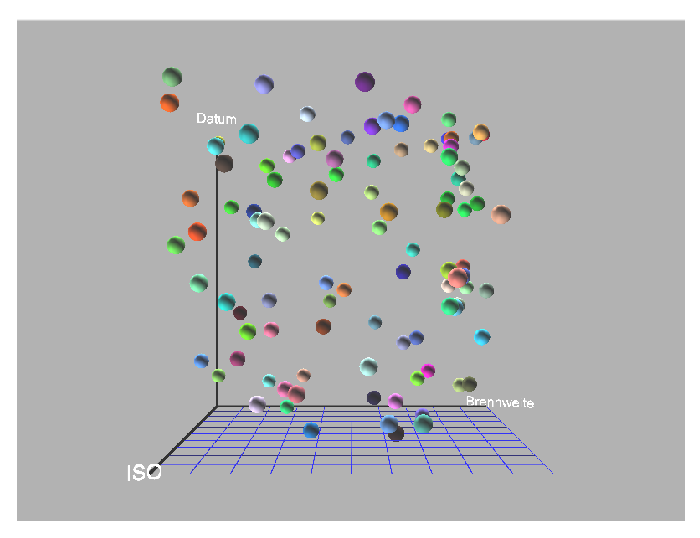
\includegraphics{images/punktewolke.eps} 
      			\caption{Ansicht einer Punktewolke}
      			\label{punktewolke}
					\end{minipage}  
    		}    		
			\end{figure}
			Die Punktewolke ist ein dreidimensionales Diagramm, bei der Punkte in einem kartesisches Koordiantensystem dargestellt werden.
			Dabei können die drei Achsen jeweils mit einem \gls{exif}-Parameter belegt werden, wobei jeder \gls{exif}-Parameter nur einmal verwendet werden darf.
			Punkte, die die gleichen Koordianten haben werden farbkodiert. Eine Farbskala gibt die Häufigkeit der individuellen Punkte an.
			Betätigt man die linken Maustaste auf einem Punkt, so wird das entsprechende Bild mit Namen angezeigt. Verbirgt sich hinter einem Punkt mehrere Bilder, so wird ein beliebiges, aber festes Bild angezeigt. 
			\par 
			
		Die Ansicht kann frei bewegt, rotiert und skaliert werden. Außerdem hat man die Möglichkeit die aktuelle Ansicht mit einem Klick auf die entsprechende Schaltfläche zurückzusetzen.
			Die Punktewolke kann als \gls{jpg} exportiert werden.

	\end{description}

\subsection{Auswertungsmanagement}

\label{subsec:auswertungsmgmt}

	Eine Auswertung ist eine Verknüpfung von beliebig (im Rahmen der \textbf{/NF020/)} vielen Bildmengen mit einem Diagrammtyp. Eine Auswertung ist dabei folgendermaßen definiert:

	\begin{itemize}

		\item Eine Auswertung kann auch ohne Auswahl von Bildmengen existieren. 

		\item Eine Auswertung hat einen frei definierbaren und vom Projektkontext abhängigen eindeutigen Namen, der zwischen einem und 200 Zeichen lang sein muss. Zu beachten ist, dass der Name automatisch um eine vorangestellte Zeichenkette ergänzt wird, die den Namen des gewählten Diagrammtyps beinhaltet.

		\item Eine Auswertung wird über eine interne ID eindeutig identifiziert.

	\end{itemize}

	Wird ein Projekt geöffnet, werden alle in der Projektkonfigurationsdatei definierten Auswertungen \gls{lexgraph} sortiert angezeigt. Die erste Auswertung der Liste (falls vorhanden), wird dabei automatisch auf aktiv gesetzt.

	\begin{description}
		
		\item[/F410/] \textit{Anlegen einer neuen Auswertung:}\par Durch betätigen der Schaltfläche "`Erstellen"' in dem Bereich "`Auswertungen"' der Projektansicht, wird ein Assistent gestartet, der den Benutzer durch die Auswertungserstellung führt.\par Über die Schaltfläche "`Vorwärts"' kann der Benutzer dabei auf den nächsten Schritt wechseln, sofern er in der aktuellen Eingabemaske keine Fehleingabe getätigt hat. Durch betätigen der Schaltfläche "`Zurück"', kann der Benutzer hingegen zu einem bereits getätigten Schritt wechseln. Auch hierbei wird vor dem Druck auf "`Vorwärts"' überprüft, ob alle Eingabedaten immer noch korrekt sind.\par Folgende Schritte führt der Assistent aus:

			\begin{enumerate}

				\item \textbf{Diagrammtyp festlegen.}

					\begin{itemize}

						\item Festlegen eines Auswertungsnamens.

						\item Eine optionale Beschreibung der Auswertung.

						\item Auswahl eines Diagrammtyps (siehe Kapitel \ref{subsec:diagrammmgmt}).\par Bei der Auswahl, wird eine Livevorschau des Diagramms mit einem Dummydatensatz angezeigt, sowie eine kurze Beschreibung über Sinn und Zweck des Diagramms.\par Hier kann auch eine bereits in dem aktiven Projekt vorhandene Auswertung, als Vorlage verwendet werden. Dabei werden alle Werte der Auswertungsvorlage übernommen, bis auf die ID und der Name. Diese beiden Werte müssen neu generiert werden, damit die Definition nicht verletzt wird.

					\end{itemize}

				\item \textbf{Parameter festlegen}.\par Festlegen der x-, y- oder z-Achse (je nach Diagrammtyp - siehe Kapitel \ref{subsec:diagrammmgmt}). Mit Festlegen ist hier das Verknüpfen mit \gls{exif}-Parametern gemeint. Optional kann eine Beschreibung angegeben werden, die dann anstatt der Bezeichnung des \gls{exif}-Parameters verwendet wird.

				\item \textbf{Bildmengen festlegen}.\par Hier werden Bildmengen des aktuell aktiven Projektes mit der Auswertung verknüpft. Außerdem kann hier anhand der \gls{exif}-Keywords eine Reduzierung der gesamten Bildmenge bewirkt werden. Dabei werden gleiche \gls{exif}-Keywords zusammengefasst. (\textit{Filterung der Daten}).

			\end{enumerate}

			Nach Beendigung des Assistenten, wird die Auswertung gespeichert und, falls bereits Bildmengen mit der Auswertung verknüpft wurden, geöffnet.
		
		\item[/F420/] \textit{Aktivieren einer Auswertung:}\par Um eine Auswertung zu aktivieren, muss man sie in der Liste der Auswertungen im Bereich "`Auswertungen"' der Projektansicht, auswählen.
		
		\item[/F430/] \textit{Bearbeiten einer Auswertung:}\par Um eine Auswertung zu bearbeiten, muss sie aktiv sein. Durch betätigen der Schaltfläche Bearbeiten"' in dem Bereich "`Auswertungen"' der Projektansicht, wird ein Dialog geöffnet, der die gleichen Auswahlmöglichkeiten des Assistenten aus \textbf{/F310/} enthält. Diese sind über Tabs auswählbar und sind mit den Werten der Auswertung vorbelegt. Nach dem Beenden des Dialogs, wird die Auswertung übernommen.
				
		\item[/F440/] \textit{Entfernen einer Auswertung:}\par Um eine Auswertung zu entfernen, muss sie aktiv sein. Durch betätigen der Schaltfläche Entfernen"' in dem Bereich "`Auswertungen"' der Projektansicht, werden folgende Aktionen ausgelöst:

			\begin{enumerate}

				\item Es wird eine Sicherheitsabfrage (ein Dialog mit Ja/Nein Auswahlmöglichkeit) angezeigt, die dem Benutzer die Möglichkeit gibt, das Entfernen abzubrechen.

				\item Die Auswertung wird aus der Liste der Auswertungen entfernt.

				\item Dem Benutzer wird eine Rückmeldung gegeben, ob das Entfernen erfolgreich war oder ob es einen Fehler gab.

				\item Nach dem Entfernen, ist die erste Auswertung (falls vorhanden) in der Liste aktiv.

			\end{enumerate}
			
	\end{description}

\subsection{Exif-Auswertung}

	\begin{description}

		\item[/F510/] \textit{Extraktion von \gls{exif} Daten:}\par Beim Einlesen von Bildern im \gls{jpg}-Format, werden nur die \gls{exif}-Parameter eingelesen, nicht die Bilddaten. Die \gls{exif}-Parameter, die verarbeitet werden, sind im Kapitel \ref{subsec:musskriterien} definiert. Die Daten werden nur während der Programmausführung intern gespeichert, dies hat zur Konsequenz, dass bei jedem Programmstart, alle \gls{exif}-Parameter neu eingelesen werden müssen (siehe Kapitel \ref{subsec:projektmanagement} \textbf{/F130/}).
	
	\end{description} \newpage
  \section{Produktdaten}

\subsection{Programmdaten}

\label{subsec:programmdaten}

\begin{description}
	
	\item[/D010/] \textit{Daten die im Programm gespeichert sind:}
	
	\begin{itemize} 
			
			\item Alle im Programm verfügbaren Projekte (in dem Projektverzeichnis - siehe Kapitel \ref{subsec:projektmanagement})
			
			\item Alle Auswertungen eines aktiven Projektes
			
			\item Alle Bildmengen eines aktiven Projektes (damit verbunden alle Pfade zu den Bildern, die in den Bildmengen liegen)
			
			\item \gls{exif}-Parameter zu jedem Bild der Bildmengen eines aktiven Projekts (siehe Kapitel \ref{subsec:musskriterien})
	
	\end{itemize}

	\item[/D020/] \textit{Daten die mit einem Projekt gespeichert werden:}
	
	\begin{itemize}
		
		\item Projekt-ID, Projektname, Projektbeschreibung, Erstellungsdatum, letztes Bearbeitungsdatum
		
		\item Alle zu einem Projekt gehörende Bildmengen, Verzeichnispfade und/oder Bildpfade
		
		\item Alle zu einem Projekt gehörenden Auswertungen
	
	\end{itemize}

	\item[/D030/] \textit{Daten die mit einer Bildmenge gespeichert werden:}
	
	\begin{itemize}
	
		\item Bildmengen-ID, Bildmengenname
		
		\item Vollständiger Pfad der zur Bildermenge gehörenden Verzeichnisse
		
		\item Vollständiger Pfad der zur Bildermenge gehörenden Bilder
		
		\item Vollständiger Pfad der Bilder, die ausgeschlossen werden sollen
	
	\end{itemize}
	
	\item[/D040/] \textit{Mit einer Auswertung gespeicherte Daten:}
	
	\begin{itemize}
		
		\item Auswertungs-ID, Auswertungsname, verknüpfte Bildmengen, \gls{exif}-Keywords, ausgewählter Diagrammtyp
		
		\item Diagrammspezifische Daten \itshape{(siehe \ref{subsec:daten-diagrammtypen})}
	
	\end{itemize}
		
\end{description}

\subsection{Daten der einzelnen Diagrammtypen}

\label{subsec:daten-diagrammtypen}

\begin{description}

	\item[/D110/] \textit{Daten des Diagrammtyps "`2D Histogramm"':}
	\begin{itemize}
		\item Ein \gls{exif}-Paramter für die x-Achse
	\end{itemize}
				
	\item[/D120/] \textit{Daten des Diagrammtyps "`3D Histogramm"':}
		\begin{itemize}
		\item Jeweils ein \gls{exif}-Paramter für die x und y-Achse
	\end{itemize}
	
	\item[/D130/] \textit{Daten des Diagrammtyps "`Boxplot"':}
		\begin{itemize}
		\item Ein \gls{exif}-Paramter für die Auswertungsgrundlage.
		\item \gls{wilcoxon}: Status, Hypothese, Signifikanzniveau
	\end{itemize}
	
	\item[/D140/] \textit{Daten des Diagrammtyps "`Punktewolke"':}
		\begin{itemize}
		\item Jeweils ein \gls{exif}-Paramter für die x,y und z-Achse
	\end{itemize}

\end{description} \newpage
  \section{Nichtfunktionale Anforderungen}

\begin{itemize}
	\item /NF10/\\Das Einlesen und extrahieren der \gls{exif} Daten sollte pro 1.000 Bildern maximal 2 Minuten und 30 Sekunden brauchen.
	\item /NF20/\\Ein Projekt muss mit einer Bildmenge von 10.000 Bildern umgehen können, ohne dass ein Programmabsturz oder längerfristigen Programmunterbrechungen daraus resultieren.
	\item /NF30/\\Bedienfehler dürfen nicht dazu führen, dass Daten verloren gehen.
	\item /NF40/\\Die grafische Benutzerschnittstelle sollte so gestaltet sein, dass ein unerfahrener Benutzer sich in angemessener Zeit einarbeiten kann.
	\item /NF50/\\ \gls{tempX} enthält nicht mehr als 1\% plattformspezifischer Anweisungen.	
	\item /NF60/\\ \gls{tempX} soll für den Startvorgang, auf dem empfohlenen System, maximal 3 Sekunden benötigen.
\end{itemize} \newpage
  \section{Globale Testfälle}

TODO: Ein Testfall für jede Anforderung. *bei Fertigstellung diese Zeile entfernen*
TODO: Testfallnummern am Ende korrigieren und den Anforderungsnummern anpassen.

\subsection{Testfälle für funktionale Anforderungen}
	
	\subsubsection{Programmausführung}
	
		\begin{description}

			\item[/F010/] \textit{Programm beenden:}\par TODO: beschreiben		
				
			\item[/T020/] \textit{Projekt speichern}\par Das in /T10/ erstellte Projekt wird gespeichert. TODO: automatisches Speichern?
				
			\item[/F030/] \textit{Automatische Anpassung der größe der Bedienoberfläsche:}\par TODO: beschreiben	
				
			\item[/F040/] \textit{Automatisches durchsuchen des Projektordners:}\par TODO: beschreiben	
		
		\end{description}

	\subsubsection{Projektmanagement}
	
		\begin{description}
		
			\item[/T110/] \textit{Neues Projekt mit einem Namen erstellen.}\par Es wird in der Projektübersicht ein neues Projekt mit dem Namen "`Schwarzwald \#3 mit Kamera \$B54\% ~n @ 3. \& 4. Berg"' erstellt.
				
			\item[/T120/] \textit{Projekt aktivieren:}\par 
				
			\item[/T130/] \textit{Gespeichertes Projekt öffnen}\par Das in \textbf{/T110/} gespeicherte Projekt wird in der Projektübersicht ausgewählt und geöffnet.
			\item[/T140/] \textit{Projekt kopieren:}\par 
				
			\item[/T150/] \textit{Projekt entfernen:}\par Das in \textbf{/T130/} geöffnete Projekt wird gelöscht.
		
		\end{description}
	
	\subsubsection{Bildmengenmanagement}
		
		\begin{description}
		
			\item[/T210/] \textit{Neue Bildmenge mit Namen erstellen.}\par
				
			\item[/T220/] \textit{Eine Bildmenge aus einer Liste auswählen.}\par

			\item[/T230/] \textit{Bildmengen per Drag \& Drop aus Bilddateien und Ordnern erzeugen.}\par
			
			\item[/F240/] \textit{Hinzufügen von Bildmengen zu einer vorhandenen Bildmenge:}\par
				
			\item[/T250/] \textit{Eine gespeicherte Bildmenge löschen.}\par
			
			\item[/T260/] \textit{Aufbau der Inhaltsliste:}\par 	
		
		\end{description}
	
	\subsubsection{Diagrammmanagement}
	
		\begin{description}
			
			\item[/T310/] \textit{Tabelle:}\par 

			\item[/T320/] \textit{Histogram 2D:}\par 
		
			\item[/T330/] \textit{Histogram 3D:}\par 

			\item[/T340/] \textit{Boxplot:}\par 

			\item[/T350/] \textit{Punktewolke:}\par 
			

			
		\end{description}
	
	\subsubsection{Auswertungsmanagement}

		\begin{description}
		
			\item[/T410/] \textit{Neue Auswertung mit Namen anlegen.}\par
			
			\item[/T420/] \textit{Eine bereits angelegte Auswertung über die Auswertungs-Liste auswählen.}\par
			
			\item[/T430/] \textit{Bearbeiten einer Auswertung:}\par 
				
			\item[/T440/] \textit{Eine Auswertung wird gelöscht.}\par
			
			TODO: fällt das nochfolgende komplett Weg? Gibt es Ersatz dafür?
			\item[/T110/] \textit{Eine Bildmenge wird einem bereits erstellten \gls{rp} hinzugefügt und wieder entfernt}\par
				
			\item[/T120/] \textit{Bildmengen werden beim Hinzufügen zum \gls{rp} über Dateinamen und \gls{exif} Daten gefiltert}\par
				
			\item[/T130/] \textit{Erstellung eines \gls{rp}s für jeden \gls{rp}-Typ.}\par
			
			\item[/T140/] \textit{Anzeige der Diagrammvorschau bei der Auswahl eines \gls{rp}s. }\par
			ENDE des nachfolgenden.
				
		\end{description}
	
	\subsubsection{Exif-Auswertung}
	
		\begin{description}

			\item[/T510/] \textit{Extraktion von \gls{exif} Daten:}\par 

		\end{description}
	
\subsection{Testfälle für nicht funktionale Anforderungen}
	
	\begin{description}
		
			\item[/T500/]\textit{10.000 Fotos mit \gls{tempX} analysieren. Für das Einlesen und Extrahieren der \gls{exif} Daten dürfen maximal 25 Minuten benötigt}\par werden.
	
	\end{description}

	\subsubsection{Testfälle für Produktumgebung}

		\begin{description}

			\item[/T510/] \textit{Extraktion von \gls{exif} Daten:}\par 

		\end{description} \newpage
  \input{PH08-Systemmodelle} \newpage
  \subsection{Szenarien}

\begin{itemize}
	\item Bernhardt arbeitet in einem Fotostudio und möchte für ein Fotoshooting am nächsten Mittwoch eine statistische Auswertung erstellen. Dabei will er feststellen, ob sich die automatische Verschlusszeit seiner Kamera mit verschiedenen \gls{Lichtformer} ändert.
	
Er öffnet \gls{tempX} und legt ein neues Projekt an. Er gibt seinem Projekt einen aussagekräftigen Namen.  Daraufhin erstellt er eine neue Auswertung, indem er auf die entsprechende Schaltfläche klickt. In dem sich öffnenden Fenster wählt er den Diagrammtypen 2D-Histogramm aus und klickt auf ''Weiter'', um den Einrichtungsassistenten zu starten. Als x-Achse wählt er ''shutter speed'' (dt.: Verschlusszeit) aus dem Aufklappmenü aus und klickt auf ''Weiter'' bis sich der Einrichtungsassistent beendet. Schließlich wird ihm angezeigt, dass er keine Bildmenge mit der aktuellen Auswertung verknüpft hat. Er klickt auf ''Speichern'' und beendet \gls{tempX}. 

\end{itemize} \newpage
  \subsection{Anwendungsfälle}

	\subsubsection{Programmmanagement:}
	\begin{description}
	\item[Anwendungsfall 1]
	\end{description}
	\begin{itemize}
		\item Name: Programm starten
		\item Teilnehmender Akteure:
		\begin{itemize}
			\item	Fotograf A.: Benutzer des Programms.
		\end{itemize}
		\item Eingangsbedingung:
		\begin{itemize}
			\item Fotograf A. besitzt das Programm.
			\item Fotograf A. hat das Programm ordnungsgemäß auf seinem PC installiert und eingerichtet.						
		\end{itemize}
		\item Ausgangsbedingung:
		\begin{itemize}
			\item	Fotograf A. hat das Programm gestartet. Es erschein das Projektverwaltungsfenster.		
		\end{itemize}
		\item Ereignisfluss:	
		\begin{itemize}
			\item Fotograf A. startet das Programm mit der ausführbaren Datei.		
			\item Das Projektverwaltungsfenster wird angezeigt.
		\end{itemize}
		\item Spezielle Anforderungen:
		\begin{itemize}
			\item	Der Computer muss den gegebenen Anforderungen genügen.
		\end{itemize}
	\end{itemize}
	\begin{description}
	\item[Anwendungsfall 2]
	\end{description}
	
	\begin{itemize}
		\item Name: Programm schließen
		\item Teilnehmender Akteure:
		\begin{itemize}
			\item	Fotograf A.: Benutzer des Programms.
		\end{itemize}
		\item Eingangsbedingung:
		\begin{itemize}
			\item Fotograf A. hat das Programm geöffnet.
			\item Fotograf A. ist fertig mit seiner Arbeit und will das Programm beenden.						
		\end{itemize}
		\item Ausgangsbedingung:
		\begin{itemize}
			\item	Fotograf A. hat das Programm beendet.		
		\end{itemize}
		\item Ereignisfluss:\\Erste Möglichkeit:	
		\begin{itemize}
			\item Fotograf A. befindet sich im Projektansichtsfenster und klickt oben rechts auf Fenster schließen.
			\item Fotograf A. hat somit das Programm beendet. Es verschwindet vom Desktop und aus den laufenden Prozessen.
		\end{itemize}
		Zweite Möglichkeit:
		\begin{itemize}
			\item Fotograf A. befindet sich nicht im Projektansichtsfenster. Daher muss er zuerst ins Projektansichtsfenster zurückkehren, indem er entweder den aktuelle Ansicht schließt oder abbricht.
			\item Fotograf A. befindet sich im Projektansichtsfenster und klickt oben rechts auf Fenster schließen.
			\item Fotograf A. hat somit das Programm beendet. Es verschwindet vom Desktop und aus den laufenden Prozessen.
		\end{itemize}	
		\item Spezielle Anforderungen:
		\begin{itemize}
			\item	Alle Eingaben müssen gültig sein.		
		\end{itemize}
	\end{itemize}
	
\begin{description}
	\item[Anwendungsfall 3]
	\end{description}
	
	\begin{itemize}
		\item Name: Programmfenster anpassen
		\item Teilnehmender Akteure:
		\begin{itemize}
			\item	Fotograf A.: Benutzer des Programms.
		\end{itemize}
		\item Eingangsbedingung:
		\begin{itemize}
			\item Fotograf A. hat das Programm geöffnet.
			\item Fotograf A. will sein Programmfenster anpassen.						
		\end{itemize}
		\item Ausgangsbedingung:
		\begin{itemize}
			\item	Fotograf A. hat das Programmfenster seinen Bedürfnissen angepasst.		
		\end{itemize}
		\item Ereignisfluss:	
		\begin{itemize}
			\item Fotograf A. kann das Programmfenster minimieren und maximieren.
			\item Fotograf A. kann das Programmfenster auf der Desktopoberfläche verschieben und positionieren.
			\item Fotograf A. kann das Programmfenster in der Höhe und Breite anpassen indem er den Rahmen mit der Maus zieht.
			\item Wenn Fotograf A. sein Programmfenster ausgerichtet hat kann er die Arbeit fortsetzen.
		\end{itemize}
		\item Spezielle Anforderungen:
		\begin{itemize}
			\item	Es muss die Mindestauflösung eingehalten werden.
			\item Die Funktionalität beschränkt sich jeweils auf die Darstellbarkeit auf dem Desktops und dem Bildschirm.
		\end{itemize}
	\end{itemize}	
	
	\subsubsection{Projektmanagement:}
		
		\# 4 \#
		\begin{itemize}
			\item Name: Erstellen eines neuen Projekts
			\item Teilnehmender Akteure:
			\begin{itemize}
				\item	Fotograf A.: Benutzer des Programms.
			\end{itemize}
			\item Eingangsbedingung:
			\begin{itemize}
				\item Fotograf A. will Bilder analysieren bzw. eine Auswertung erstellen.						
			\end{itemize}
			\item Ausgangsbedingung:
			\begin{itemize}
				\item	Fotograf A. hat ein Projekt, mit welchem er arbeiten kann.		
			\end{itemize}
			\item Ereignisfluss:
			\begin{itemize}
				\item Fotograf A. startet das Programm auf seinem Computer.
				\item Fotograf A. bekommt das Projektverwaltungsfenster angezeigt. Es befindet sich entweder noch kein Projekt in der Liste oder es sind bereits Projekte vorhanden.
				\item Fotograf A. klickt auf Neues Projekt erstellen.
				\item Es erscheint ein Fenster mit Textfeld.
				\item Fotograf A. gibt einen gültigen Namen für sein Projekt ein.
				\item Fotograf A. bestätigt seine Eingabe.
				\item Fotograf A. gelangt in das Projektansichtsfenster seines Projekts und kann mit seinem Vorhaben beginnen. Ihm wird der Projektname links oben angezeigt.
				\item In Zukunft wird der Name des Projekts auch in der Liste der Projekte mit aufgenommen.
			\end{itemize}
			\item Spezielle Anforderungen:
			\begin{itemize}
				\item	Das Programm muss korrekt auf dem PC eingerichtet sein.
				\item Alle Eingaben müssen korrekt sein.
			\end{itemize}			
		\end{itemize}
		
		\# 5 \#
		\begin{itemize}
			\item Name: Entfernen eines Projekts
			\item Teilnehmender Akteure:
			\begin{itemize}
				\item	Fotograf A.: Benutzer des Programms.	
			\end{itemize}
			\item Eingangsbedingung:
			\begin{itemize}
				\item	Das Programm befindet sich im Projektverwaltungsfenster.		
			\end{itemize}
			\item Ausgangsbedingung:
			\begin{itemize}
				\item	Ein ausgewähltes Projekt wird aus dem Programm und vom Computer entfernt.		
			\end{itemize}
			\item Ereignisfluss:
			\begin{itemize}
				\item Fotograf A. klickt auf das Projekt welches er entfernen will um es zu markieren.
				\item Fotograf A. klickt auf den Button Projekt entfernen.
				\item Fotograf A.	bestätigt Sicherheitsabfrage mit Ja.
				\item Das Projekt verschwindet aus der Liste.
			\end{itemize}
			\item Spezielle Anforderungen:
			\begin{itemize}
				\item	Es existiert mindestens ein Projekt.		
			\end{itemize}			
		\end{itemize}
		
		\# 6 \#
		\begin{itemize}
			\item Name: Öffnen eines Projekts
			\item Teilnehmender Akteure:
			\begin{itemize}
				\item	Fotograf A.: Benutzer des Programms.		
			\end{itemize}
			\item Eingangsbedingung:
			\begin{itemize}
				\item	Das Programm befindet sich im Projektverwaltungsfenster.
				\item Es ist bereits mindestens ein Projekt in der Projektliste vorhanden.
			\end{itemize}
			\item Ausgangsbedingung:
			\begin{itemize}
				\item	Ein bereits erstelltes Projekt ist vollständig geladen und wird Fotograf A. angezeigt. Es kann bearbeitet werden.		
			\end{itemize}
			\item Ereignisfluss:\\Erste Möglichkeit:
			\begin{itemize}
				\item Fotograf A. klickt einmal auf das zu öffnende Projekt um es zu markieren.
				\item Fotograf A. klickt auf Button Projekt öffnen um zum Projekt zu gelangen.
				\item Das Projekt wird im Projektansichtsfenster angezeigt.
			\end{itemize}
			Zweite Möglichkeit:
			\begin{itemize}
				\item Fotograf A. klickt per Doppelklick direkt aud Projektnamen um es direkt zu öffnen.
				\item Das Projekt wird im Projektansichtsfenster angezeigt.					
			\end{itemize}
			\item Spezielle Anforderungen:
			\begin{itemize}
				\item	Es existiert bereits mindestens ein Projekt.	
			\end{itemize}			
		\end{itemize}
		
		\# 7 \#
		\begin{itemize}
			\item Name: Kopieren eines Projekts
			\item Teilnehmender Akteure:
			\begin{itemize}
				\item	Fotograf A.: Benutzer des Programms		
			\end{itemize}
			\item Eingangsbedingung:
			\begin{itemize}
				\item	Das Programm befindet sich im Projektverwaltungsfenster.
				\item Es ist bereits mindestens ein Projekt in der Projektliste vorhanden.			
			\end{itemize}
			\item Ausgangsbedingung:
			\begin{itemize}
				\item	Es wurde ein neues Projekt erstellt, welches die selben Eigenschaften und Daten enthält wie ein anderes.	
			\end{itemize}
			\item Ereignisfluss:
			\begin{itemize}
				\item Fotograf A. klickt einmal auf das zu kopierende Projekt um es zu markieren.
				\item Fotograf A. klickt auf den Button Projekt kopieren.
				\item Es erscheint ein Fenster mit Textfeld.
				\item Fotograf A. gibt einen gültigen Namen für sein Projekt ein.
				\item Fotograf A. bestätigt seine Eingabe.
				\item Fotograf A. gelangt in das Projektansichtsfenster seines eben erstellten Projekts und kann mit seiner Arbeit beginnen. Ihm wird der Projektname links oben angezeigt.
				\item Alle Werte und Einstellungen werden vom Originalobjekt übernommen und auch dementsprechend angezeigt.
			\end{itemize}
			\item Spezielle Anforderungen:
			\begin{itemize}
				\item	Es existiert bereits mindestens ein Projekt.		
			\end{itemize}			
		\end{itemize}

	\subsubsection{Bildmengenmanagement:}
	
	\# 8 \#
	\begin{itemize}
		\item Name: Erstellen einer Bildmenge
		\item Teilnehmender Akteure:
		\begin{itemize}
			\item	Fotograf A.: Benutzer des Programms		
		\end{itemize}
		\item Eingangsbedingung:
		\begin{itemize}
			\item	Das Programm befindet sich im Projektansichtsfenster eines aktiven Projekts.
			\item Fotograf A. will eine neue Bildmenge erstellen und dieser Bilder zuweisen.
		\end{itemize}
		\item Ausgangsbedingung:
		\begin{itemize}
			\item	Es wurde eine neue Bildmenge erstellt welche Bilder enthält.	
		\end{itemize}
		\item Ereignisfluss:
		\begin{itemize}
			\item Fotograf A. klickt im Projektansichtsfenster im Bereich der Bildmengen auf "`Erstellen"'.		
			\item Nun erscheint ein neues Fenster, indem oben in einem Textfeld einen Namen eingetragen werden kann.
			\item Fotograf A. gibt einen gültigen Namen für seine Bildermenge ein.
			\item Im unteren Teil des Fensters befindet sich links
			\item Es erscheint ein Fenster mit Textfeld.
			\item Fotograf A. gibt einen gültigen Namen für sein Projekt ein.
			\item Fotograf A. bestätigt seine Eingabe.
			\item Fotograf A. gelangt in das Projektansichtsfenster seines eben erstellten Projekts und kann mit seiner Arbeit beginnen. Ihm wird der Projektname links oben angezeigt.
			\item Alle Werte und Einstellungen werden vom Originalobjekt übernommen und auch dementsprechend angezeigt.
		\end{itemize}
		\item Spezielle Anforderungen:
		\begin{itemize}
			\item	Es existiert bereits mindestens ein Projekt.		
		\end{itemize}			
	\end{itemize}
 \newpage
  \input{PH08c-Objektmodell} \newpage
  \input{PH08d-Dynamische_Modelle} \newpage
  \input{PH08e-Benutzerschnittstelle} \newpage
  %+++Workaround++++++++++++++++++++++++++++++++++++++++++++++++++++++++++++++++++++++++++++++++++++

% Durch diesen Workaround, wird das Glossar in der TOC und auf der Seite richtig nummeriert
\stepcounter{section}
\addcontentsline{toc}{section}{\numberline {\thesection} Glossar}

%+++Ausgabe+++++++++++++++++++++++++++++++++++++++++++++++++++++++++++++++++++++++++++++++++++++++

% Schreibt das Glossar
\printglossary[style=list,title=\thesection~Glossar]
\end{document}
